\documentclass[tikz,border=3pt]{standalone}
\usepackage{amsmath,amssymb}
\usetikzlibrary{arrows.meta,calc}
\definecolor{curveblue}{HTML}{245C86}
\definecolor{accent}{HTML}{A65E2E}
\definecolor{curveteal}{HTML}{287B6D}
\definecolor{curveviolet}{HTML}{76578B}
\begin{document}
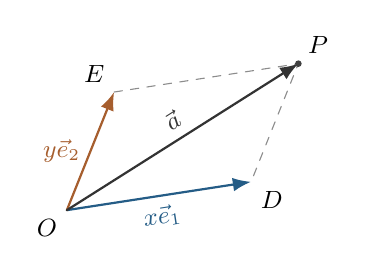
\begin{tikzpicture}[font=\small,>=Latex,line cap=round,line join=round]

\coordinate (O) at (0,0); \coordinate (D) at (2.34,.36);
\coordinate (E) at (.60,1.50); \coordinate (P) at (2.94,1.86);
\draw[->,curveblue,thick] (O)--node[below,sloped]{$x\vec e_1$}(D);
\draw[->,accent,thick] (O)--node[left]{$y\vec e_2$}(E);
\draw[black!45,dashed] (E)--(P)--(D);
\draw[->,black!80,thick] (O)--node[above,sloped]{$\vec a$}(P);
\node[below left] at (O) {$O$};\node[below right] at (D) {$D$};
\node[above left] at (E) {$E$};\node[above right] at (P) {$P$};
\fill[black!75] (P) circle (1.2pt);
\end{tikzpicture}
\end{document}
